\section{Exercise 3 - Combining \texttt{MPI} Processes}

PROPER ZITAT ZU AUFGABE 5

With the goal of saving slightly on communication rounds by combining a pipelined reduction and a 
pipelined broadcast more tightly to keep the processes “more busy”, we end up with the function implementation 
of \texttt{MY\_Allreduce\_P()}. This implementation is completely based on the pipelined tree 
implementation for exercise 5 (REFER HERE TO EX5). For better understanding, refer to exercise 5 first.\\

Hence, we interpret the “lined up” processes as a tree, where each node except one leaf has exactly 
one child and all nodes except the root have a parent node. With this understanding, we reuse the 
implementation of \texttt{MY\_Allreduce\_T()} from exercise 5 by getting rid of the communication between 
a “right child” and it’s parent as in our setting for exercise 3 only “left children” exist.\\

We can expect an improvement compared to the trivial combination of \texttt{MY\_Reduce\_P()} and 
\texttt{MY\_Bcast\_P()}, as in \texttt{MY\_Allreduce\_P()} the reduction already gets started as soon 
as the data of the first block received the master process -- the root node. Therefore, 
$\text{number of processes/nodes} - 1 + \text{number of blocks}$ are needed in \texttt{MY\_Allreduce\_P()}, 
whereas \texttt{MY\_Reduce\_P()} and \texttt{MY\_Bcast\_P()} use $\text{number of blocks}$ communication rounds 
each. For a small numbers of processes/nodes, the number of communication rounds can be reduced based 
on the number of blocks and therefore the blocksize.\\

\begin{figure}[h]
    \begin{center}
        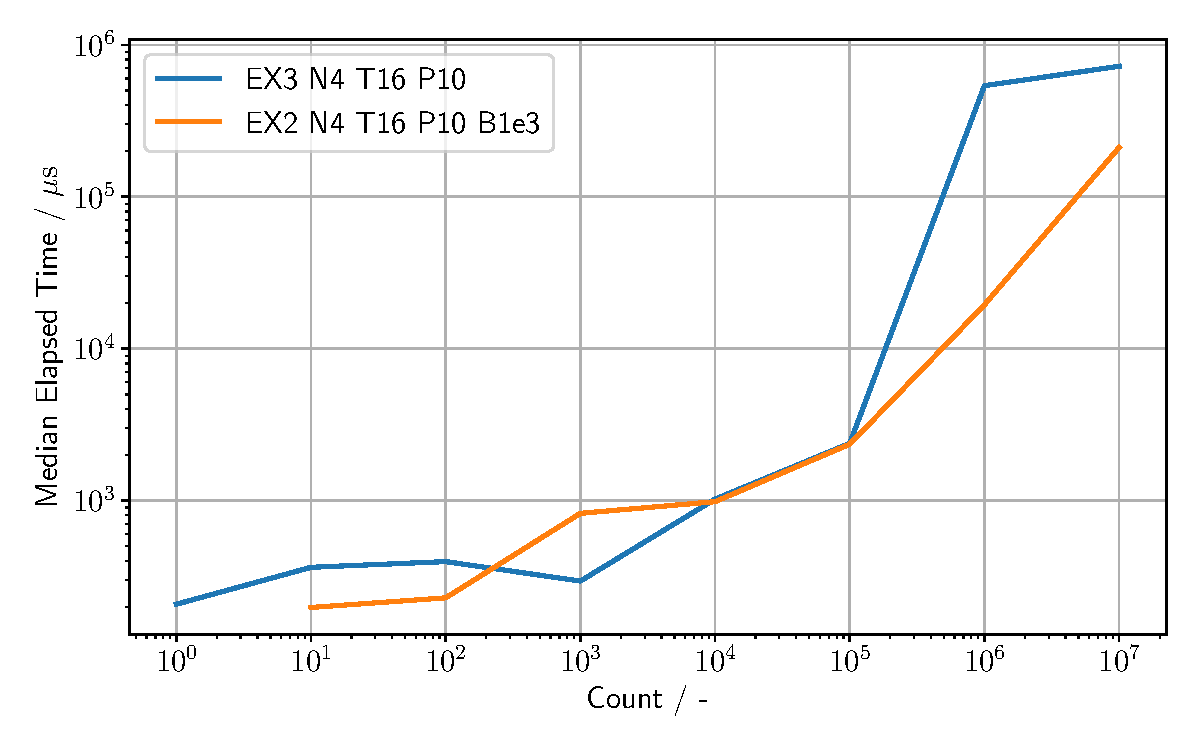
\includegraphics[width=1.0\linewidth]{figures/Ex3_1.pdf}
        \caption{Caption for Ex3 plot 1}
        \label{Ex3_1_p}
    \end{center}
\end{figure}

\begin{figure}[h]
    \begin{center}
        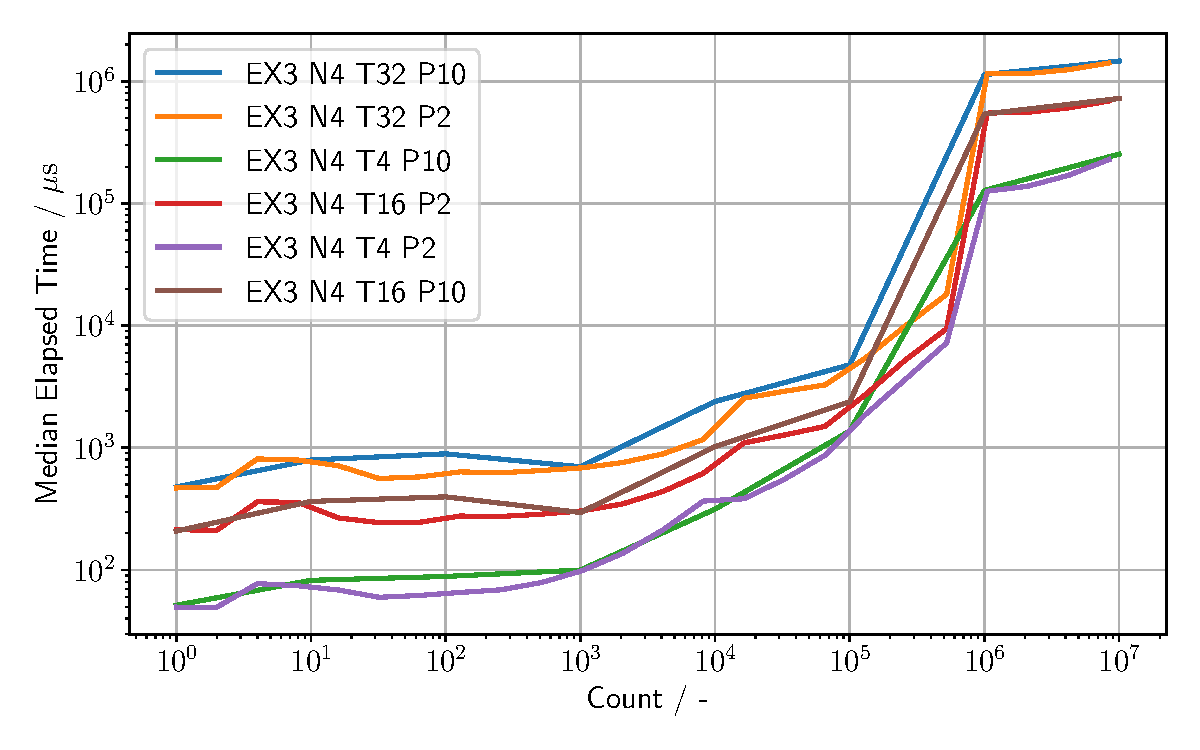
\includegraphics[width=1.0\linewidth]{figures/Ex3_2.pdf}
        \caption{Caption for Ex3 plot 2}
        \label{Ex3_2_p}
    \end{center}
\end{figure}

\begin{figure}[h]
    \begin{center}
        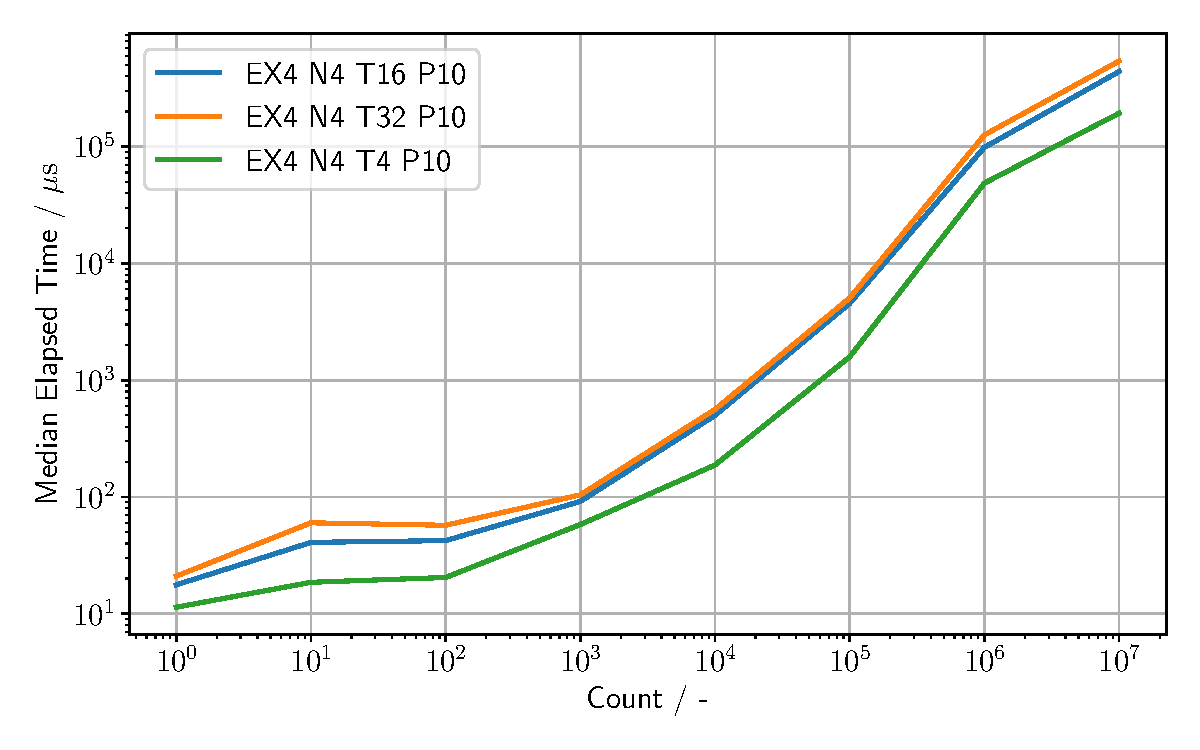
\includegraphics[width=1.0\linewidth]{figures/Ex3_3.pdf}
        \caption{Caption for Ex3 plot 3}
        \label{Ex3_3_p}
    \end{center}
\end{figure}